\RequirePackage[l2tabu, orthodox]{nag}
\RequirePackage{silence}
\WarningFilter{fmtcount}{\ordinal already defined use \FCordinal instead}
\documentclass[english, french]{beamer}
%Permits to copy eg x ⪰ y iff v(x) ≥ v(y) from PDF to unicode data. 
	\pdfgentounicode=1 % TODO these two do not seem to have any effect
	\input{glyphtounicode}
%Latin Modern has more glyphs than Computer Modern, such as diacritical characters, and permits copy from resulting PDF. fntguide commands to load the font before fontenc, to prevent default loading of cmr.
	\usepackage{lmodern}
%Encode resulting accented characters correctly in resulting PDF, permits copy from PDF.
	\usepackage[T1]{fontenc}
%UTF8 seems to be the default in recent TeX installations, but not all, see https://tex.stackexchange.com/a/370280.
	\usepackage[utf8]{inputenc}
%Provides \newunicodechar for easy definition of supplementary UTF8 characters such as → or ≤ for use in source code.
	\usepackage{newunicodechar}
%Text Companion fonts, much used together with CM-like fonts. Provides \texteuro and other similar commands for text mode characters such as \textminus, \textrightarrow, \textlbrackdbl.
	\usepackage{textcomp}
%Solves bug in lmodern, https://tex.stackexchange.com/a/261188; probably useful only for unusually big font sizes.
	%\DeclareFontShape{OMX}{cmex}{m}{n}{
		%<-7.5> cmex7
		%<7.5-8.5> cmex8
		%<8.5-9.5> cmex9
		%<9.5-> cmex10
	%}{}
	%\SetSymbolFont{largesymbols}{normal}{OMX}{cmex}{m}{n}
	%\SetSymbolFont{largesymbols}{bold}  {OMX}{cmex}{m}{n}
%More symbols (such as \sum) available in bold version, see https://github.com/latex3/latex2e/issues/71.
	\DeclareFontShape{OMX}{cmex}{bx}{n}{%
	   <->sfixed*cmexb10%
	   }{}
	\SetSymbolFont{largesymbols}{bold}{OMX}{cmex}{bx}{n}
%There’s no bold small caps in Latin Modern, we switch to Computer Modern for bold small caps, see https://tex.stackexchange.com/a/22241
	%\normalfont\DeclareFontShape{T1}{lmr}{bx}{sc} { <-> ssub * cmr/bx/sc }{}
%Warn about missing characters.
	\tracinglostchars=2
%Nicer tables: provides \toprule, \midrule, \bottomrule.
	%\usepackage{booktabs}
%For new column type X which stretches; can be used together with booktabs, see https://tex.stackexchange.com/a/97137.
	%\usepackage{tabularx}
%Provides \addtocmd, \patchcmd, \newtoggle commands. xpatch extends etoolbox.
	\usepackage{xpatch} 
%ntheorem doc says: “empheq provides an enhanced vertical placement of the endmarks”; must be loaded before ntheorem. Loads the mathtools package, which loads and fixes some bugs in amsmath and provides \DeclarePairedDelimiter. TODO amsmath is considered a basic, mandatory package nowadays (Grätzer, More Math Into LaTeX).
	\usepackage[ntheorem]{empheq}
%Package frenchb asks to load natbib before babel-french. Package hyperref asks to load natbib before hyperref.
	\usepackage{natbib}

\newtoggle{LCpres}
	\makeatletter
	\@ifclassloaded{beamer}{
		\toggletrue{LCpres}
		\wlog{Presentation mode}
	}{
		\togglefalse{LCpres}
		\wlog{Article mode}
	}
	\makeatother%

%Language options ([french, english]) should be on the document level (last is main); except with tikzposter: put [french, english] options next to \usepackage{babel} to avoid warning. beamer uses the \translate command for the appendix: omitting babel results in a warning, see https://github.com/josephwright/beamer/issues/449. Babel also seems required for \refname.
	\iftoggle{LCpres}{
		\usepackage{babel}
	}{
	}
	%\frenchbsetup{AutoSpacePunctuation=false}
%listings (1.7) does not allow multi-byte encodings. listingsutf8 works around this only for characters that can be represented in a known one-byte encoding and only for \lstinputlisting. Other workarounds: use literate mechanism; or escape to LaTeX (but breaks alignment).
	\usepackage{listings}
	\lstset{tabsize=2, basicstyle=\ttfamily, escapechar=§, literate={é}{{\'e}}1, aboveskip=0pt}
%I favor acro over acronym because the former is more recently updated (2018 VS 2015 at time of writing); has a longer user manual (about 40 pages VS 6 pages if not counting the example and implementation parts); has a command for capitalization; and acronym suffers a nasty bug when ac used in section, see https://tex.stackexchange.com/q/103483 (though this might be the fault of the silence package and might be solved in more recent versions, I do not know). However, loading it makes compilation time (one pass on this template) go from 0.6 to 1.4 seconds, see https://bitbucket.org/cgnieder/acro/issues/115. Option short-format not usable in the package options as it is fragile, see https://tex.stackexchange.com/q/466882.
	%\usepackage[single]{acro}
	%\acsetup{short-format = {\scshape}}
	%\DeclareAcronym{AMCD}{short=amcd, long={Aide Multicritère à la Décision}}
\DeclareAcronym{AR}{short=ar, long={Argumentative Recommender}}
\DeclareAcronym{DA}{short=da, long={Decision Analysis}}
\DeclareAcronym{DJ}{short=dj, long={Deliberated Judgment}}
\DeclareAcronym{DM}{short=dm, long={Decision Maker}}
\DeclareAcronym{DP}{short=dp, long={Deliberated Preference}}
\DeclareAcronym{MAVT}{short=mavt, long={Multiple Attribute Value Theory}}
\DeclareAcronym{MCDA}{short=mcda, long={Multicriteria Decision Aid}}
\DeclareAcronym{MIP}{short=mip, long={Mixed Integer Program}}


\iftoggle{LCpres}{
	%I favor fmtcount over nth because it is loaded by datetime anyway; and fmtcount warns about possible conflicts when loaded after nth.
	\usepackage{fmtcount}
	%For nice input of date of presentation. Must be loaded after the babel package. Has possible problems with srcletter: https://golatex.de/verwendung-von-babel-und-datetime-in-scrlttr2-schlaegt-fehlt-t14779.html.
	\usepackage[nodayofweek]{datetime}
}{
}
%For presentations, Beamer implicitely uses the pdfusetitle option. ntheorem doc says to load hyperref “before the first use of \newtheorem”. autonum doc mandates option hypertexnames=false. I want to highlight links only if necessary for the reader to recognize it as a link, to reduce distraction. In presentations, this is already taken care of by beamer. If using colorlinks=true in a presentation, see https://tex.stackexchange.com/q/203056.
\makeatletter
\iftoggle{LCpres}{
	\usepackage{hyperref}
}{
	\usepackage[hypertexnames=false, pdfusetitle, linkbordercolor={1 1 1}, citebordercolor={1 1 1}, urlbordercolor={1 1 1}]{hyperref}
	%https://tex.stackexchange.com/a/466235
	\pdfstringdefDisableCommands{%
		\let\thanks\@gobble
	}
}
\makeatother
%urlbordercolor is used both for \url and \doi, which I think shouldn’t be colored, and for \href, thus might want to color manually when required. Requires xcolor.
	\newcommand{\hrefblue}[2]{\textcolor{blue}{\href{#1}{#2}}}
%hyperref doc says: “Package bookmark replaces hyperref’s bookmark organization by a new algorithm (...) Therefore I recommend using this package”.
	\usepackage{bookmark}
%Need to invoke hyperref explicitly to link to line numbers: \hyperlink{lintarget:mylinelabel}{\ref*{lin:mylinelabel}}, with \ref* to disable automatic link. Also see https://tex.stackexchange.com/q/428656 for referencing lines from another document.
	%\usepackage{lineno}
	%\newcommand{\llabel}[1]{\hypertarget{lintarget:#1}{}\linelabel{lin:#1}}
	%\setlength\linenumbersep{9mm}
%For complex authors blocks. Seems like authblk wants to be later than hyperref, but sooner than silence.
	\nottoggle{LCpres}{
		\usepackage{authblk}
		\renewcommand\Affilfont{\small}
		%TODO https://tex.stackexchange.com/a/471297 (no effect here!)
		\xpretocmd{\author}{\addhrauthor{#2}}{}{}
		\newif\iffirstauthor
		\firstauthortrue
		\newcommand{\addhrauthor}[1]{%
			\iffirstauthor%
				\newcommand{\hrauthor}{#1}\firstauthorfalse%
			\else%
				\xapptocmd{\hrauthor}{, #1}{}{}%
			\fi
		}
	}{
	}
%I do not use floatrow, because it requires an ugly hack for proper functioning with KOMA script (see scrhack doc). Instead, the following command centers all floats (using \centering, http://texblog.net/latex-archive/layout/center-centering/), and I manually place my table captions above and figure captions below their contents (https://tex.stackexchange.com/a/3253).
	\makeatletter
	\g@addto@macro\@floatboxreset\centering
	\makeatother
%Permits to customize enumeration display and references
	%\nottoggle{LCpres}{
		%\usepackage{enumitem} %follow enumerate by a string to customize enumeration
	%}{
	%}
%Provides \Cen­ter­ing, \RaggedLeft, and \RaggedRight and en­vi­ron­ments Cen­ter, FlushLeft, and FlushRight, which al­low hy­phen­ation. With tikzposter, seems to cause 1=1 to be printed in the middle of the poster.
	%\usepackage{ragged2e}
%To typeset units by closely following the “official” rules.
	%\usepackage[strict]{siunitx}
%Turns the doi provided by some bibliography styles into URLs. However, uses old-style dx.doi url (see 3.8 DOI system Proxy Server technical details, “Users may resolve DOI names that are structured to use the DOI system Proxy Server (https://doi.org (current, preferred) or earlier syntax http://dx.doi.org).”, https://www.doi.org/doi_handbook/3_Resolution.html). The patch solves this.
	\usepackage{doi}
	\makeatletter
	\patchcmd{\@doi}{http://dx.doi.org}{https://doi.org}{}{}
	\makeatother
%Makes sure upper case greek letters are italic as well.
	\usepackage{fixmath}
%Provides \mathbb; obsoletes latexsym (see http://tug.ctan.org/macros/latex/base/latexsym.dtx). Relatedly, \usepackage{eucal} to change the mathcal font and \usepackage[mathscr]{eucal} (apparently equivalent to \usepackage[mathscr]{euscript}) to supplement \mathcal with \mathscr. This last option is not very useful as both fonts are similar, and the intent of the authors of eucal was to provide a replacement to mathcal (see doc euscript). Also provides \mathfrak for supplementary letters.
	\usepackage{amsfonts}
%Provides a beautiful (IMHO) \mathscr and really different than \mathcal, for supplementary uppercase letters. But there is no bold version.
	\usepackage{mathrsfs}
%Multiple means to produce bold math: \mathbf, \boldmath (defined to be \mathversion{bold}, see fntguide), \pmb, \boldsymbol (all legacy, from LaTeX base and AMS), \bm (the most recommended one), \mathbold from package fixmath (I don’t see its advantage over \boldsymbol).
%“The \boldsymbol command is obtained preferably by using the bm package, which provides a newer, more powerful version than the one provided by the amsmath package. Generally speaking, it is ill-advised to apply \boldsymbol to more than one symbol at a time.” — AMS Short math guide. “If no bold font appears to be available for a particular symbol, \bm will use ‘poor man’s bold’” — bm. It is “best to load the package after any packages that define new symbol fonts” – bm. bm defines \boldsymbol as synonym to \bm. \boldmath accesses the correct font if it exists; it is used by \bm when appropriate. See https://tex.stackexchange.com/a/10643 and https://github.com/latex3/latex2e/issues/71 for some difficulties with \bm.
	\usepackage{bm}
	\nottoggle{LCpres}{
	%https://ctan.org/pkg/amsmath recommends ntheorem, which supersedes amsthm, which corrects the spacing of proclamations and allows for theoremstyle. Option standard loads amssymb and latexsym. Must be loaded after amsmath (from ntheorem doc). From cleveref doc, “ntheorem is fully supported and even recommended”; says to load cleveref after ntheorem.
		\usepackage[thmmarks, amsmath, standard, hyperref]{ntheorem}
		%empheq doc says to do this after loading ntheorem
		\usetagform{default}
	%Provides \cref. Unfortunately, cref fails when the language is French and referring to a label whose name contains a colon (https://tex.stackexchange.com/q/83798). Use \cref{sec\string:intro} to work around this. cleveref should go “laster” than hyperref.
		\usepackage{cleveref}
	%Equations get numbers iff they are referenced. Loading order should be “amsmath → hyperref → cleveref → autonum”, according to autonum doc. Use this in preference to the showonlyrefs option from mathtools, see https://tex.stackexchange.com/q/459918 and autonum doc. See https://tex.stackexchange.com/a/285953 for the etex line.
		\expandafter\def\csname ver@etex.sty\endcsname{3000/12/31}\let\globcount\newcount
		\usepackage{autonum}
	}{
	}
%Also loaded by tikz.
	%\usepackage{xcolor}
\iftoggle{LCpres}{
	\usepackage{tikz}
	%\usetikzlibrary{babel, matrix, fit, plotmarks, calc, trees, shapes.geometric, positioning, plothandlers, arrows, shapes.multipart}
}{
}
%Vizualization, on top of TikZ
	%\usepackage{pgfplots}
	%\pgfplotsset{compat=1.14}
\usepackage{graphicx}
	\graphicspath{{graphics/}}

%Provides \print­length{length}, useful for debugging.
	%\usepackage{printlen}
	%\uselengthunit{mm}
%Provides \NewDocumentCommand and similar commands possibly intended as replacement of \newcommand in LaTeX3 (for package authors? see https://tex.stackexchange.com/q/98152 and https://github.com/latex3/latex2e/issues/89).
	%\usepackage{xparse}

\iftoggle{LCpres}{
	%“fixes the frame num­ber­ing in beamer when us­ing an ap­pendix such that the slides from the ap­pendix are not counted in the to­tal frame num­ber of the main part of the doc­u­ment”. Maybe not necessary with recent versions of Beamer, see https://tex.stackexchange.com/a/133175.
		\usepackage{appendixnumberbeamer}
	%I have yet to see anyone actually use these navigation symbols – this command removes them.
		\setbeamertemplate{navigation symbols}{}
%\usetheme{CambridgeUS}
	\usepackage{preamble/beamerthemeParisFrance}
}{
}


\NewDocumentCommand{\R}{}{ℝ}
\NewDocumentCommand{\N}{}{ℕ}
%\mathscr is rounder than \mathcal.
\NewDocumentCommand{\powerset}{m}{\mathscr{P}(#1)}
%Powerset without zero.
\NewDocumentCommand{\powersetz}{m}{\mathscr{P}^*(#1)}
%https://tex.stackexchange.com/a/45732, works within both \set and \set*, same spacing than \mid (https://tex.stackexchange.com/a/52905).
\NewDocumentCommand{\suchthat}{}{\;\ifnum\currentgrouptype=16 \middle\fi|\;}
%Integer interval.
\NewDocumentCommand{\intvl}{m}{⟦#1⟧}
%Allows for \abs and \abs*, which resizes the delimiters.
\DeclarePairedDelimiter\abs{\lvert}{\rvert}
\DeclarePairedDelimiter\card{\lvert}{\rvert}
\DeclarePairedDelimiter\floor{\lfloor}{\rfloor}
\DeclarePairedDelimiter\ceil{\lceil}{\rceil}
%Perhaps should use U+2016 ‖ DOUBLE VERTICAL LINE here?
\DeclarePairedDelimiter\norm{\lVert}{\rVert}
%From mathtools. Better than using the package braket because braket introduces possibly undesirable space. Then: \begin{equation}\set*{x \in \R^2 \suchthat \norm{x}<5}\end{equation}.
\DeclarePairedDelimiter\set{\{}{\}}
\DeclareMathOperator*{\argmax}{arg\,max}
\DeclareMathOperator*{\argmin}{arg\,min}

%UTR #25: Unicode support for mathematics recommend to use the straight form of phi (by default, given by \phi) rather than the curly one (by default, given by \varphi), and thus use \phi for the mathematical symbol and not \varphi. I however prefer the curly form because the straight form is too easy to mix up with the symbol for empty set.
\let\phi\varphi

%The amssymb solution.
%\NewDocumentCommand{\restr}{mm}{{#1}_{\restriction #2}}
%Another acceptable solution.
%\NewDocumentCommand{\restr}{mm}{{#1|}_{#2}}
%https://tex.stackexchange.com/a/278631; drawback being that sometimes the text collides with the line below.
\NewDocumentCommand\restr{mm}{#1\raisebox{-.5ex}{$|$}_{#2}}


%Voting and MCDA
\newcommand{\allalts}{\mathscr{A}}
\newcommand{\alts}{A}
\newcommand{\allF}{\mathcal{F}}
\newcommand{\cat}[1]{C_{#1}}

%Voting
\newcommand{\feasalts}{F}
\newcommand{\allvoters}{\mathscr{N}}
\newcommand{\voters}{N}
\newcommand{\allsystems}{\mathcal{G}}
\newcommand{\prof}{\mathbf{R}}
\newcommand{\allprofs}{\mathbfcal{R}}
\newcommand{\linors}{\mathcal{L}(\alts)}

\newcommand{\pbasic}[1]{\prof^{#1}_\epsilon}
\newcommand{\pelem}[1]{\prof^{#1}_e}
\newcommand{\pcycl}[1]{\prof^{#1}_c}
\newcommand{\pcycllong}[1]{\prof^{#1}_{cl}}
\newcommand{\pinv}[1]{\overline{\prof_{#1}}}
\newcommand{\dmap}{{\xitsfamily δ}}
%powerset without zero
\newcommand{\powersetz}[1]{\mathcal{P}_\emptyset(#1)}

%logic atom
%⟼ (long)
\DeclareDocumentCommand{\lato}{ O{\prof} O{\alts} }{[#1 \!⟼\! #2]}
%logic atom in
%↝, \stackrel{\in}{\mapsto}, ➲, ⥹
\newcommand{\tightoverset}[2]{%
  \mathop{#2}\limits^{\vbox to -.5ex{\kern-0.9ex\hbox{$#1$}\vss}}}
\DeclareDocumentCommand{\latoin}{ O{\prof} O{\alpha} }{[#1 \tightoverset{\in}{⟼} #2]}
\newcommand{\alllang}{\mathcal{L}}
\newcommand{\ltru}{\texttt{T}}
\newcommand{\lfal}{\texttt{F}}
\newcommand{\laxiom}[1]{{\texgyreherosfamily{\textsc{#1}}}}

%ARG TH
\newcommand{\AF}{\mathcal{AF}}
\newcommand{\labelling}{\mathcal{L}}
\newcommand{\labin}{\textbf{in}\xspace}
\newcommand{\labout}{\textbf{out}}
\newcommand{\labund}{\textbf{undec}\xspace}
\newcommand{\nonemptyor}[2]{\ifthenelse{\equal{#1}{}}{#2}{#1}}
\newcommand{\gextlab}[2][]{
	\labelling{\mathcal{GE}}_{(#2, \nonemptyor{#1}{\ibeatsr{#2}})}
}
\newcommand{\allargs}{A^*}
\newcommand{\args}{A}
\newcommand{\ar}{a}
\newcommand{\ext}{\mathcal{E}}

%MCDA+Arg
\newcommand{\dm}{d}
\newcommand{\ileadsto}{\rightcurvedarrow}
\newcommand{\mleadsto}[1][\eta]{\rightcurvedarrow_{#1}}
\newcommand{\ibeats}{\vartriangleright}
\newcommand{\mbeats}[1][\eta]{\vartriangleright_{#1}}

%MISC
\newcommand{\lequiv}{\Vvdash}
\newcommand{\weightst}{W^{\,t}}

%MCDA classical
\newcommand{\crits}{\mathcal{J}}

%Sorting
\newcommand{\cats}{\mathcal{C}}
\newcommand{\catssubsets}{2^\cats}
\newcommand{\catgg}{\vartriangleright}
\newcommand{\catll}{\vartriangleleft}
\newcommand{\catleq}{\trianglelefteq}
\newcommand{\catgeq}{\trianglerighteq}
\newcommand{\alttoc}[2][x]{(#1 \xrightarrow{} #2)}
\newcommand{\alttocat}[3]{(#2 \xrightarrow{#1} #3)}
\newcommand{\alttoI}{(x \xrightarrow{} \left[\underline{C_x}, \overline{C_x}\right])}
\newcommand{\alttocatdm}[3][t]{\left(#2 \thinspace \raisebox{-3pt}{$\xrightarrow{#1}$}\thinspace #3\right)}
\newcommand{\alttocatatleast}[2]{\left(#1 \thinspace \raisebox{-3pt}{$\xrightarrow[]{≥}$}\thinspace #2\right)}
\newcommand{\alttocatatmost}[2]{\left(#1 \thinspace \raisebox{-3pt}{$\xrightarrow[]{≤}$}\thinspace #2\right)}

\newcommand{\source}{\scriptsize}
\newcommand{\commentOC}[1]{{\selectlanguage{french}{\todo{OC : #1}}}}
%Or: \todo[color=green!40]

%this probably requires outdated float package, see doc KomaScript for an alternative.
% \newfloat{program}{t}{lop}
% \floatname{program}{PM}

%\crefname{axiom}{axiom}{axioms}%might be needed for workaround bug in cref when defining new theorems?

%\ifdefined\theorem\else
%\newtheorem{theorem}{\iflanguage{english}{Theorem}{Théorème}}
%\fi

%which line breaks are chosen: accept worse lines, therefore reducing risk of overfull lines. Default = 200
\tolerance=2000
%accept overfull hbox up to...
\hfuzz=2cm
%reduces verbosity about the bad line breaks
\hbadness 5000
%sloppy sets tolerance to 9999
\apptocmd{\sloppy}{\hbadness 10000\relax}{}{}

% WRITING
%\newcommand{\ie}{i.e.\@\xspace}%to try
%\newcommand{\eg}{e.g.\@\xspace}
%\newcommand{\etal}{et al.\@\xspace}
\newcommand{\ie}{i.e.\ }
\newcommand{\eg}{e.g.\ }
\newcommand{\mkkOK}{\checkmark}%\color{green}{\checkmark}
\newcommand{\mkkREQ}{\ding{53}}%requires pifont?%\color{green}{\checkmark}
\newcommand{\mkkNO}{}%\text{\color{red}{\textsf{X}}}

\makeatletter
\newcommand{\boldor}[2]{%
	\ifnum\strcmp{\f@series}{bx}=\z@
		#1%
	\else
		#2%
	\fi
}
\newcommand{\textstyleElProm}[1]{\boldor{\MakeUppercase{#1}}{\textsc{#1}}}
\makeatother
\newcommand{\electre}{\textstyleElProm{Électre}\xspace}
\newcommand{\electreIv}{\textstyleElProm{Électre Iv}\xspace}
\newcommand{\electreIV}{\textstyleElProm{Électre IV}\xspace}
\newcommand{\electreIII}{\textstyleElProm{Électre III}\xspace}
\newcommand{\electreTRI}{\textstyleElProm{Électre Tri}\xspace}
% \newcommand{\utadis}{\texorpdfstring{\textstyleElProm{utadis}\xspace}{UTADIS}}
% \newcommand{\utadisI}{\texorpdfstring{\textstyleElProm{utadis i}\xspace}{UTADIS I}}

%TODO
% \newcommand{\textstyleElProm}[1]{{\rmfamily\textsc{#1}}} 

\newcommand{\menuit}{\emph}

%Usage: \jeeref{javax.persistence/EntityManager} ; \jeeref[@]{javax.persistence/PersistenceContextType\#EXTENDED}
\newcommand{\jeeref}[2][]{\japiref{https://docs.oracle.com/javaee/7/api/}{#1}{#2}}
\newcommand{\jseref}[2][]{\japiref{https://docs.oracle.com/javase/8/docs/api/}{#1}{#2}}
\newcommand{\japiref}[3]{%
	\edef\refAPIBaseUrl{#1}%
	\edef\refAPIAnnot{#2}%
	\IfSubStr{#3}{\#}{%
		\StrBefore{#3}{\#}[\refAPIFQName]%
		\StrBehind{#3}{\#}[\refAPIField]%
		\edef\refAPIFieldLink{\#\refAPIField}%
		\edef\refAPIFieldShow{.\refAPIField}%
	}{%
		\edef\refAPIFQName{#3}%
		\edef\refAPIField{}%
		\edef\refAPIFieldLink{}%
		\edef\refAPIFieldShow{}%
	}%
	\StrBefore{\refAPIFQName}{/}[\refAPIPackage]%
	\StrBehind{\refAPIFQName}{/}[\refAPIClass]%
	\StrSubstitute{\refAPIPackage}{.}{/}[\refAPIPackageSlashes]%
%	annot: \refAPIAnnot%
%	\\fqname: \refAPIFQName%
%	\\field: \refAPIFieldLink%
%	\\package: \refAPIPackageSlashes%
%	\\class: \refAPIClass%
	\IfEq{\refAPIField}{}{%
		\href{%
			\refAPIBaseUrl\refAPIPackageSlashes/\refAPIClass.html\refAPIFieldLink%
		}{%
			\texttt{\refAPIAnnot\refAPIClass}%
		}%
	}{%
		\texttt{\refAPIAnnot\refAPIClass.}%
		\href{%
			\refAPIBaseUrl\refAPIPackageSlashes/\refAPIClass.html\refAPIFieldLink%
		}{%
			\texttt{\refAPIField}%
		}%
	}%
}


%const
\newcommand{\tikzboxit}{\path node[draw, overlay, inner sep=0.6mm, fit=(boxed), rectangle] {};}%

\newlength{\GraphsNodeSep}
\setlength{\GraphsNodeSep}{7mm}

% MCDA Drawing Sorting
\newlength{\MCDSCatHeight}
\setlength{\MCDSCatHeight}{6mm}
\newlength{\MCDSAltHeight}
\setlength{\MCDSAltHeight}{4mm}
%separation between two vertical alts
\newlength{\MCDSAltSep}
\setlength{\MCDSAltSep}{2mm}
\newlength{\MCDSCatWidth}
\setlength{\MCDSCatWidth}{3cm}
\newlength{\MCDSAltWidth}
\setlength{\MCDSAltWidth}{2.5cm}
\newlength{\MCDSEvalRowHeight}
\setlength{\MCDSEvalRowHeight}{6mm}
\newlength{\MCDSAltsToCatsSep}
\setlength{\MCDSAltsToCatsSep}{1.5cm}
\newcounter{MCDSNbAlts}
\newcounter{MCDSNbCats}
\newlength{\MCDSArrowDownOffset}
\setlength{\MCDSArrowDownOffset}{0mm}

\tikzset{/Graphs/dot/.style={
	shape=circle, fill=black, inner sep=0, minimum size=1mm
}}
\tikzset{/MC/D/S/alt/.style={
	shape=rectangle, draw=black, inner sep=0, minimum height=\MCDSAltHeight, minimum width=\MCDSAltWidth
}}
\tikzset{MC/D/S/pref/.style={
	shape=ellipse, draw=gray, thick
}}
\tikzset{/MC/D/S/cat/.style={
	shape=rectangle, draw=black, inner sep=0, minimum height=\MCDSCatHeight, minimum width=\MCDSCatWidth
}}
\tikzset{/MC/D/S/evals matrix/.style={
	matrix, row sep=-\pgflinewidth, column sep=-\pgflinewidth, nodes={shape=rectangle, draw=black, inner sep=0mm, text depth=0.5ex, text height=1em, minimum height=\MCDSEvalRowHeight, minimum width=12mm}, nodes in empty cells, matrix of nodes, inner sep=0mm, outer sep=0mm, row 1/.style={nodes={draw=none, minimum height=0em, text height=, inner ysep=1mm}}
}}

\newlength{\GitCommitSep}
\setlength{\GitCommitSep}{13mm}

\tikzset{/Git/commit/.style={
	shape=rectangle, draw, minimum width=4em, minimum height=0.6cm
}}
\tikzset{/Git/branch/.style={
	shape=ellipse, draw, red
}}
\tikzset{/Git/head/.style={
	shape=ellipse, draw, fill=yellow
}}

\tikzset{profile matrix/.style={
	matrix of math nodes, column sep=3mm, row sep=2mm, nodes={inner sep=0.5mm, anchor=base}
}}
\tikzset{rank-profile matrix/.style={
	matrix of math nodes, column sep=3mm, row sep=2mm, nodes={anchor=base}, column 1/.style={nodes={inner sep=0.5mm}}, row 1/.style={nodes={inner sep=0.5mm}}
}}
\tikzset{rank-vector/.style={
	draw, rectangle, inner sep=0, outer sep=1mm
}}
\tikzset{isolated rank-vector/.style={
	draw, matrix of math nodes, column sep=3mm, inner sep=0, matrix anchor=base, nodes={anchor=base, inner sep=.33em}, ampersand replacement=\&
}}

% GUI
\tikzset{/GUI/button/.style={
	rectangle, very thick, rounded corners, draw=black, fill=black!40%, top color=black!70, bottom color=white
}}

% Logger objects
\tikzset{/logger/main/.style={
	shape=rectangle, draw=black, inner sep=1ex, minimum height=7mm
}}
\tikzset{/logger/helper/.style={
	shape=rectangle, draw=black, dashed, minimum height=7mm
}}
\tikzset{/logger/helper line/.style={
	<->, draw, dotted
}}

% Beliefs
\tikzset{/Beliefs/D/S/attacker/.style={
	shape=rectangle, draw, minimum size=8mm
}}
\tikzset{/Beliefs/D/S/supporter/.style={
	shape=circle, draw
}}

\newcommand{\tikzmark}[1]{%
	\tikz[overlay, remember picture, baseline=(#1.base)] \node (#1) {};%
}


\DeclareAcronym{AMCD}{short=amcd, long={Aide Multicritère à la Décision}}
\DeclareAcronym{AR}{short=ar, long={Argumentative Recommender}}
\DeclareAcronym{DA}{short=da, long={Decision Analysis}}
\DeclareAcronym{DJ}{short=dj, long={Deliberated Judgment}}
\DeclareAcronym{DM}{short=dm, long={Decision Maker}}
\DeclareAcronym{DP}{short=dp, long={Deliberated Preference}}
\DeclareAcronym{MAVT}{short=mavt, long={Multiple Attribute Value Theory}}
\DeclareAcronym{MCDA}{short=mcda, long={Multicriteria Decision Aid}}
\DeclareAcronym{MIP}{short=mip, long={Mixed Integer Program}}


%this approach does not generalize to multipart nodes.
%\tikzset{/uml/interface/.style={rectangle, draw, fill=yellow!20, align=left, node font=\fontspec{Latin Modern Mono Light}, node contents={$<<$interface$>>$\\\textbf{#1}}, name=#1
%}}
%this approach does not apply for <<interface>>. Never mind, I’ll do it manually, as I can’t find anything better. Use: \nodepart[font=]{one} \small <<interface>>\\\bfseries ItemDAO
\tikzset{/uml/class/.style={rectangle, draw, align=center, fill=yellow!20, node font=\fontspec{Latin Modern Mono Light}, font=\bfseries
}}
\tikzset{/uml/abstract class/.style={rectangle, draw, align=center, fill=yellow!20, node font=\fontspec{Latin Modern Mono Light}, font=\bfseries\itshape
}}
\tikzset{/uml/class3/.style={
rectangle split, rectangle split every empty part={}, rectangle split parts=3, rectangle split part align={center, left, left}, draw, fill=yellow!20, rectangle split empty part height=0, node font=\fontspec{Latin Modern Mono Light}, every one node part/.style={font=\bfseries, align=center}, every two node part/.style={align=left}, every three node part/.style={align=left}
}}
\tikzset{/uml/extends/.style={draw, -open triangle 45}}
\tikzset{/uml/implements/.style={draw, -open triangle 45, dashed}}
%prefix= used to cancel \texttt, otherwise this cancels the effect of the font selection \fontspec{Latin Modern Mono Light}, and thus renders \bfseries inoperant. With prefix=, the result is correct.
%\jeeref[prefix=]{javax.faces.component.html/HtmlCommandButton}\\
\tikzset{/uml/table/.style={rectangle, draw, align=center, fill=blue!20, node font=\fontspec{Latin Modern Mono Light}, font=\bfseries
}}
\tikzset{/uml/table2/.style={
rectangle split, rectangle split every empty part={}, rectangle split parts=2, rectangle split part align={center, left}, draw, fill=blue!20, rectangle split empty part height=0, node font=\fontspec{Latin Modern Mono Light}, every one node part/.style={font=\bfseries, align=center}, every two node part/.style={align=left}
}}
\tikzset{/uml/dbkey/.style={draw, ->}}
%http://tex.stackexchange.com/questions/79781/placing-anchor-before-and-after-text-in-multipart-rectangle



\setbeamertemplate{headline}[singleline]

\title{Git}
\subject{Git}
\keywords{VCS, SCM, version control}
\author{Olivier Cailloux}
\institute[LAMSADE]{LAMSADE, Université Paris-Dauphine}
\date{Version du \today}

\begin{document}
\bibliographystyle{apalike}

\begin{frame}[plain]
	\tikz[remember picture,overlay]{
		\path (current page.south west) node[anchor=south west, inner sep=0] {
			\includegraphics[height=1cm]{LAMSADE95.jpg}
		};
		\path (current page.south) ++ (0, 1mm) node[anchor=south, inner sep=0] {
			\includegraphics[height=9mm]{Dauphine.jpg}
		};
		\path (current page.south east) node[anchor=south east, inner sep=0] {
			\includegraphics[height=1cm]{PSL.png}
		};
	}
   \titlepage
\end{frame}
\addtocounter{framenumber}{-1}

\section{Présentation}
\begin{frame}
	\frametitle{Git}
	\begin{itemize}
		\item Contrôle de version (VCS, SCM) : conserver l’historique
		\item Pour tous types de projet : code, images, présentations, article…
		\item VCS local, centralisé, distribué ? \pause
		\item Centralisé : seulement sur un serveur distant
		\item Distribué : copie locale et distante
		\item Git : distribué
	\end{itemize}
\end{frame}

\section{Commits}
\begin{frame}
	\frametitle{Commits et historique}
	\begin{itemize}
		\item Blob : capture d’un fichier à un moment donné
		\item Commit : identifié par un hash SHA-1
		\begin{itemize}
			\item Contient : structure de répertoires ; \emph{blobs} ; auteur…
		\end{itemize}
		\item Histoire : un DAG de \og{}commits\fg{}
	\end{itemize}
	{
		\centering
		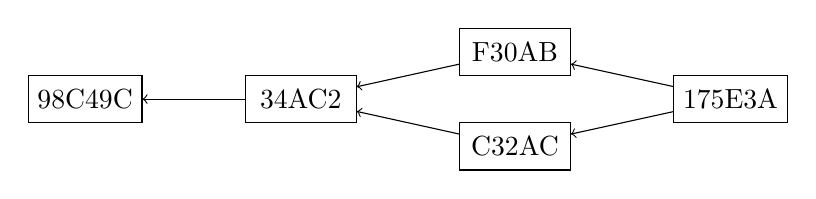
\begin{tikzpicture}
			\path node[/Git/commit] (c1) {98C49C};
			\path (c1.east) ++ (\GitCommitSep, 0) node[anchor=west, /Git/commit] (c2) {34AC2} edge[->] (c1);
			\path (c2.east) ++ (\GitCommitSep, 6mm) node[anchor=west, /Git/commit] (c3N) {F30AB} edge[->] (c2);
			\path (c2.east) ++ (\GitCommitSep, -6mm) node[anchor=west, /Git/commit] (c3S) {C32AC} edge[->] (c2);
			\path (c2 -| c3N.east) ++ (\GitCommitSep, 0) node[anchor=west, /Git/commit] (c4) {175E3A} edge[->] (c3N) edge[->] (c3S);
		\end{tikzpicture}\par
	}
\end{frame}

\begin{frame}
	\frametitle{Work dir (WD)}
	\begin{itemize}
		\item Histoire conservée \emph{localement} dans \texttt{.git} à la racine du projet
		\item WD (\og{}work dir\fg{}) : version du projet (fichiers et sous-répert.)
		\item Interaction avec sous-rép. \texttt{.git} : \emph{uniquement} via outils git
	\end{itemize}
	\texttt{/root}
	\begin{itemize}
		\item[] \texttt{/.git}
		\item[] \texttt{/rép1}
		\begin{itemize}
			\item[] \texttt{/fich1}
		\end{itemize}\vspace{-0.8ex}
		\item[] \texttt{/fich2}
	\end{itemize}
\end{frame}

\begin{frame}
	\frametitle{Préparer un commit}
	\begin{minipage}[t]{0.33 \columnwidth}
		\textbf{Work dir}
		\begin{itemize}
%			\item[] \texttt{/.git}
			\item[] \texttt{/rép1}
			\begin{itemize}
				\item[] \texttt{/fich1}
			\end{itemize}\vspace{-0.8ex}
			\item[] \texttt{/fich2}
			\item[] \texttt{/fich3}
		\end{itemize}
	\end{minipage}%
	\begin{minipage}[t]{0.33 \columnwidth}
		\textbf{Index}
		\begin{itemize}
			\item[] \texttt{/rép1}
			\begin{itemize}
				\item[] \texttt{/fich1'}
			\end{itemize}\vspace{-0.8ex}
			\item[] \texttt{/fich2}
		\end{itemize}
	\end{minipage}%
	\begin{minipage}[t]{0.33 \columnwidth}
		\textbf{HEAD}
		\begin{itemize}
			\item[] \texttt{/rép1}
			\begin{itemize}
				\item[] \texttt{/fich1}
			\end{itemize}\vspace{-0.8ex}
			\item[] \texttt{/fich2'}
		\end{itemize}
	\end{minipage}
	\begin{itemize}
		\item \emph{Index} : changements à apporter au prochain commit
		\item \emph{HEAD} : commit d’où le work dir actuel est issu
		\item Initialisation nouveau répertoire ? \pause Index et HEAD vide \pause
		\item Juste après un commit ? \pause Index vide
	\end{itemize}
\end{frame}

\begin{frame}
	\frametitle{Préparer un commit : définitions}
%	\small
	\begin{minipage}[t]{0.33 \columnwidth}
		\textbf{Work dir}
		\begin{itemize}
%			\item[] \texttt{/.git}
			\item[] \texttt{/rép1}
			\begin{itemize}
				\item[] \texttt{/fich1}
			\end{itemize}\vspace{-0.8ex}
			\item[] \texttt{/fich2}
%			\item[] \texttt{/fich3}
		\end{itemize}
	\end{minipage}%
	\begin{minipage}[t]{0.33 \columnwidth}
		\textbf{Index}
		\begin{itemize}
			\item[] \texttt{/rép1}
			\begin{itemize}
				\item[] \texttt{/fich1'}
			\end{itemize}\vspace{-0.8ex}
			\item[] \texttt{/fich2}
		\end{itemize}
	\end{minipage}%
	\begin{minipage}[t]{0.33 \columnwidth}
		\textbf{HEAD}
		\begin{itemize}
			\item[] \texttt{/rép1}
			\begin{itemize}
				\item[] %\texttt{/fich1}
			\end{itemize}\vspace{-0.8ex}
			\item[] \texttt{/fich2'}
		\end{itemize}
	\end{minipage}
	\begin{block}{Définitions (étant donné un fichier)}
	%nb on devrait peut-être appliquer modified et unmodified seulement pour les \emph{tracked}. Auquel cas on peut aussi définir :\item[\emph{modified}] [{∈} index ⇒ ≠ index] ; [{∉} index ⇒ {∈} HEAD ∧ ≠ HEAD]. Donc modified implique tracked.
		\begin{description}[\emph{unmodified}]
			\item[{∈} index] blob ds index, peut être ≠ WD
			\item[∈ HEAD] blob ds HEAD, peut être ≠ WD
			\item[\emph{untracked}] [{∉} index] et [{∉} HEAD]
			\item[\emph{tracked}] [{∈} index] ou [{∈} HEAD] {\tiny (ou les deux)}
			\item[\emph{modified}] [{∈} index ⇒ ≠ index] ; [{∉} index ⇒ ≠ HEAD]
			\item[\emph{unmodified}] [{∈} index ⇒ = index] ; [{∉} index ⇒ = HEAD]
		\end{description}
	\end{block}
\end{frame}

\begin{frame}
	\frametitle{Préparer un commit : commandes}
%	\begin{block}{Commandes}
		\begin{itemize}\setlength{\itemindent}{-1em}
			\item \texttt{git add fichier} : blob mis dans index (\og{}staged\fg{})
			\item \emph{clean} WD : tous {\tiny (sauf fichiers dans gitignore)} tracked et unmodified
			\item \texttt{git status} : liste untracked, {\tiny tracked-}modified, staged
			\item \texttt{git status -{}-short} {\tiny (sauf merge conflict)} : idx VS HEAD ; WD VS idx.
			\item \texttt{git diff} : WD VS index
			\item \texttt{git diff -{}-staged} : index VS HEAD
			\item \texttt{git commit} : commenter et expédier ! (Renvoie son id SHA-1)
			\item \texttt{git commit -v} : voir l’index en détail
		\end{itemize}
%	\end{block}
\end{frame}

\section{Branches}
\begin{frame}
	\frametitle{Branches et HEAD}
	\begin{itemize}
		\item Branche : pointeur vers un commit
		\item HEAD : pointeur vers {\tiny (typiquement)} une branche\\et un commit
		\item Branche \og{}actuelle\fg{}\\désignée par HEAD
	\end{itemize}
	\begin{tikzpicture}[overlay]
		\path (3.7cm, 0) node[/Git/commit] (c1) {98C49C};
		\path (c1.east) ++ (\GitCommitSep, 0) node[anchor=west, /Git/commit] (c2) {34AC2} edge[->] (c1);
		\path (c2.east) ++ (\GitCommitSep, 0) node[anchor=west, /Git/commit] (c3) {F30AB} edge[->] (c2);
		\path (c2.north) ++ (0, 3mm) node[anchor=south, /Git/branch] (master) {master} edge[->] (c2);
		\path (c3.north) ++ (0, 3mm) node[anchor=south, /Git/branch] (br) {br} edge[->] (c3);
		\path (br.north) ++ (0, 3mm) node[anchor=south, /Git/head] (head) {HEAD} edge[->] (br);
	\end{tikzpicture}
	\vspace{3mm}
	\begin{itemize}
		\item commit : avance HEAD et branche actuelle
		\item \texttt{git branch truc} : crée branche \texttt{truc}. HEAD inchangé !
		\item \texttt{git checkout truc} : change HEAD et met à jour WD
		\item Conseil : WD clean avant checkout !
		\item \texttt{git log -{}-graph -{}-decorate -{}-oneline -{}-all}
	\end{itemize}
\end{frame}

\begin{frame}
	\frametitle{Fusion de branches}
	{
	\centering
	\begin{tikzpicture}
		\path (3.7cm, 0) node[/Git/commit] (c1) {98C49C};
		\path (c1.east) ++ (\GitCommitSep, 0) node[anchor=west, /Git/commit] (c2) {34AC2} edge[->] (c1);
		\path (c2.east) ++ (\GitCommitSep, 4mm) node[anchor=west, /Git/commit] (c3N) {F30AB} edge[->] (c2);
		\path (c2.east) ++ (\GitCommitSep, -4mm) node[anchor=west, /Git/commit] (c3S) {C32AC} edge[->] (c2);
		\path (c2.north) ++ (0, 3mm) node[anchor=south, /Git/branch] (master) {master} edge[->] (c2);
		\path (c3N.north) ++ (0, 3mm) node[anchor=south, /Git/branch] (br) {br} edge[->] (c3N);
		\path (br.north) ++ (0, 3mm) node[anchor=south, /Git/head] (head) {HEAD} edge[->] (br);
	\end{tikzpicture}\par
	}
	\begin{itemize}
		\item \texttt{git merge autrebranche} : fusionne changements de \texttt{autrebranche} dans branche actuelle
		\item Si \texttt{autrebranche} est en avant de l’actuelle : \og{}fast-forward\fg{}
		\item Sinon, \og{}merge conflict\fg{} possible. Modifier les fichiers à la main et les ajouter à l’index puis commit pour créer un merge.
		\item checkout d’un commit {\tiny (ou tag)} sans branche {\tiny (detached head state)} : lecture !
	\end{itemize}
\end{frame}

\section{Serveurs distants}
\begin{frame}
	\frametitle{Serveurs distants}
	\vspace{-1pt}
	\begin{itemize}
		\item Réf. distante (\og{}remote ref\fg{}) : pointeurs vers branches {\tiny et tags} sur dépots distants
		\item \og{}Remote-tracking branch\fg{} : branche locale correspondant à une branche distante et qui connait l’état de la branche distante correspondante la dernière fois qu’on l’a vue
		\item Remote \og{}origin\fg{} supposé configuré ici
		\item \texttt{git branch -vv} : voir branches et correspondants distants
		\item \texttt{git fetch} : récupère les commits distants ; met à jour (ou crée) les références distantes
		\item \texttt{git push origin mabranche} : sinon, nouvelles branches restent locales
		\item \texttt{git remote show origin} : voir les réf. distantes
		\item Suivre une branche distante : checkout \texttt{origin/branche} ; créer branche locale ; \texttt{git branch -{}-set-upstream-to origin/branch}
	\end{itemize}
\end{frame}

\section{Divers}
\begin{frame}
	\frametitle{Divers}
	\vspace{-1pt}
	\begin{itemize}
		\item Utilisez gitignore {\tiny (\href{https://github.com/github/gitignore}{modèles})}
		\item Créez-vous une paire clé publique / privée
		\item Raccourcis : à éviter au début
		\item \texttt{git init} : dépôt vide dans rép. courant (rien n’est traqué)
		\item \texttt{git clone url} : cloner un dépôt (et non checkout !)
		\item \texttt{git stash} : WD $←$ HEAD
		\item \texttt{git tag -a montag} {\tiny (tag annoté, recommandé)} puis \texttt{git push origin montag}
		\item \texttt{git config -{}-global} : écrit dans \texttt{\textasciitilde/.gitconfig}
		\item Indiquez propriété \texttt{user.name} (et \texttt{user.email})
		\item Déterminer des \href{https://git-scm.com/book/en/v2/Git-Tools-Revision-Selection}{révisions} {\tiny exemple : HEAD\textasciicircum 1 pour parent de HEAD}
		\item \href{https://git-scm.com/book/en/v2/Git-Basics-Git-Aliases}{Alias}
		\item \href{https://git-scm.com/book/en/v2}{Documentation}
		\item GUI pour diff : \texttt{git difftool}
		\item GUI pour merge : \texttt{git mergetool}
	\end{itemize}
\end{frame}

\section{Références}
\begin{frame}
	\frametitle{Références}
	\begin{itemize}
		\item \href{https://git-scm.com/downloads}{Téléchargement} officiel
		\item \href{https://git-scm.com/book/}{Livre} Pro Git
		\item \href{https://try.github.io/}{tryGit}
	\end{itemize}
\end{frame}

\section{Exercices}
\begin{frame}[allowframebreaks]
	\small
	\frametitle{Exercices : Git}
	Git en local
	\begin{itemize}
		\item Définir globalement (au moins) \texttt{user.name}. Vérifier avec \texttt{git config -{}-list}.
		\item Créer un répertoire projet et dedans un fichier \texttt{début.txt} contenant \texttt{"coucou"}.
		\item Initialiser un dépôt git dans ce projet.
		\item Placer \texttt{début.txt} dans l’index. Modifier \texttt{début.txt} pour qu’il contienne \texttt{"coucou2"}. Visualiser la différence sur ce fichier entre la version WD, index, et dépôt. Faire en sorte que le blob dans l’index contienne bien \texttt{"coucou2"}.
		\item Effectuer un premier commit, qui contiendra uniquement \texttt{début.txt}. À l’issue de ce commit, vérifier que vous obtenez l’historique suivant.\par
		{
			\centering
			\begin{tikzpicture}
				\path node[/Git/commit] (c1) {C1};
				\path (c1.north) ++ (0, 3mm) node[anchor=south, /Git/branch] (master) {master} edge[->] (c1);
				\path (master.north) ++ (0, 3mm) node[anchor=south, /Git/head] (head) {HEAD} edge[->] (master);
			\end{tikzpicture}\par
		}
		\item Vous avez maintenant une idée audacieuse pour résoudre un problème dans votre projet. Comme vous n’êtes pas sûr de sa pertinence, vous désirez placer vos changements dans une nouvelle branche en attendant d’y réfléchir. Créer une branche \texttt{"dev"} ; y commettre un fichier \texttt{audacieux.txt} (en plus de \texttt{début.txt}, inchangé) contenant \texttt{"approche 1"}. Votre historique doit maintenant être celui-ci (vérifier !).\par
		{
			\centering
			\begin{tikzpicture}
				\path node[/Git/commit] (c1) {C1};
				\path (c1.north) ++ (0, 3mm) node[anchor=south, /Git/branch] (master) {master} edge[->] (c1);
				\path (c1.east) ++ (\GitCommitSep, 0) node[anchor=west, /Git/commit] (c2) {C2} edge[->] (c1);
				\path (c2.north) ++ (0, 3mm) node[anchor=south, /Git/branch] (dev) {dev} edge[->] (c2);
				\path (dev.north) ++ (0, 3mm) node[anchor=south, /Git/head] (head) {HEAD} edge[->] (dev);
			\end{tikzpicture}\par
		}
		\item À l’issue de ce travail harrassant, il vous vient une idée alternative. N’étant toujours pas sûr de la valeur de votre première idée (dans \texttt{dev}), vous repartirez de \texttt{master} pour l’implémenter. Depuis \texttt{master}, créer une branche \texttt{dev2}, et y commettre (en plus de \texttt{début.txt}, inchangé) un fichier \texttt{audacieux.txt} contenant \texttt{"approche alternative"}. Vérifier ensuite votre historique.\par
		{
			\centering
			\begin{tikzpicture}
				\path node[/Git/commit] (c1) {C1};
				\path (c1.north) ++ (0, 3mm) node[anchor=south, /Git/branch] (master) {master} edge[->] (c1);
				\path (c1.east) ++ (\GitCommitSep, 4mm) node[anchor=west, /Git/commit] (c2) {C2} edge[->] (c1);
				\path (c2.north) ++ (0, 2mm) node[anchor=south, /Git/branch] (dev) {dev} edge[->] (c2);
				\path (c1.east) ++ (\GitCommitSep, -4mm) node[anchor=west, /Git/commit] (c3) {C3} edge[->] (c1);
				\path (c3.south) ++ (0, -2mm) node[anchor=north, /Git/branch] (dev2) {dev2} edge[->] (c3);
				\path (dev2.south) ++ (0, -2mm) node[anchor=north, /Git/head] (head) {HEAD} edge[->] (dev2);
			\end{tikzpicture}\par
		}
		\item À la réflexion, votre première idée est bonne. L’intégrer dans \texttt{master} pour obtenir l’historique suivant. Prédire si vous obtiendrez un fast-forward et vérifier.\par
		{
			\centering
			\begin{tikzpicture}
				\path node[/Git/commit] (c1) {C1};
				\path (c1.east) ++ (\GitCommitSep, 4mm) node[anchor=west, /Git/commit] (c2) {C2} edge[->] (c1);
				\path (c2.north) ++ (0, 3mm) node[anchor=south, /Git/branch] (master) {master} edge[->] (c2);
				\path (master.west) ++ (-5mm, 0) node[anchor=east, /Git/branch] (dev) {dev} edge[->] (c2);
				\path (c1.east) ++ (\GitCommitSep, -4mm) node[anchor=west, /Git/commit] (c3) {C3} edge[->] (c1);
				\path (c3.south) ++ (0, -2mm) node[anchor=north, /Git/branch] (dev2) {dev2} edge[->] (c3);
				\path (master.north) ++ (0, 2mm) node[anchor=south, /Git/head] (head) {HEAD} edge[->] (master);
			\end{tikzpicture}\par
		}
		\item Tout bien réfléchi vous aimez également votre deuxième idée. L’intégrer à son tour dans \texttt{master} et obtenir cet historique. Quel problème allez-vous rencontrer, ce faisant ?\par
		{
			\centering
			\begin{tikzpicture}
				\path node[/Git/commit] (c1) {C1};
				\path (c1.east) ++ (\GitCommitSep, 4mm) node[anchor=west, /Git/commit] (c2) {C2} edge[->] (c1);
				\path (c1.east) ++ (\GitCommitSep, -4mm) node[anchor=west, /Git/commit] (c3) {C3} edge[->] (c1);
				\path (c1 -| c2.east) ++ (\GitCommitSep, 0) node[anchor=west, /Git/commit] (c4) {C4} edge[->] (c2) edge[->] (c3);
				\path (c4.north) ++ (0, 3mm) node[anchor=south, /Git/branch] (master) {master} edge[->] (c4);
				\path (master.north) ++ (0, 2mm) node[anchor=south, /Git/head] (head) {HEAD} edge[->] (master);
			\end{tikzpicture}\par
		}
		\item Imaginons qu’on aurait d’abord intégré \texttt{dev2} à \texttt{master} (ceci aurait-il produit un fast-forward ?) puis \texttt{dev} au résultat. Quel aurait été le résultat final ?
	\end{itemize}
	\framebreak
	Git distant
	\begin{itemize}
		\item Cloner votre dépôt central pour le projet de ce cours (ou votre dépôt local).
		\item Le clonage vous a créé un pointeur vers un serveur distant \texttt{origin}, et une \og{}remote-tracking branch\fg{} \texttt{master}. Voir où pointent \texttt{origin}, \texttt{master} et \texttt{origin/master}.
		\item Ajouter un fichier \texttt{"macontrib.txt"} contenant votre prénom à votre index local. Commettre dans votre dépôt git local. L’envoyer au dépôt distant. Vérifier (via l’interface web) qu’il s’y trouve et que le commit est associé à votre nom.
		\item Quand un collègue a fait de même, vous pouvez rapatrier sa modification en local. Après l’avoir fait, prédire où vont pointer \texttt{master} et \texttt{origin/master} et vérifier.
		\item Si un collègue a publié sa modification avant la vôtre, quel va être votre problème ? Comment le résoudre ? Si vous êtes le premier à publier la modification, allez aider vos collègues à publier la leur !
	\end{itemize}
\end{frame}


\appendix
\AtBeginSection{
}

\section{Licence}
\begin{frame}
	\frametitle{Licence}
	Cette présentation, et le code LaTeX associé, sont sous \href{http://opensource.org/licenses/MIT}{licence MIT}. Vous êtes libres de réutiliser des éléments de cette présentation, sous réserve de citer l’auteur.
	
	Le travail réutilisé est à attribuer à \href{http://www.lamsade.dauphine.fr/~ocailloux/}{Olivier Cailloux}, Université Paris-Dauphine.
	
	\small{(Ceci ne couvre pas les images incluses dans ce document, puisque je n’en suis généralement pas l’auteur.)}
\end{frame}
\end{document}

\begin{frame}
	\frametitle{}
	\begin{itemize}
		\item 
	\end{itemize}
	\begin{block}{}
		
	\end{block}
\end{frame}

\section{Bibliographie}
\begin{frame}[allowframebreaks]
	\frametitle{Bibliographie}
	\def\newblock{\hskip .11em plus .33em minus .07em}
% 	\bibliography{zotero}
\end{frame}

\section{Autres}
\begin{frame}
	\frametitle{}
	\begin{itemize}
		\item 
	\end{itemize}
	\begin{block}{}
		
	\end{block}
\end{frame}
\end{document}
